\section{\texorpdfstring{\epsolute{}}{Epsolute}}\label{section:range-persistent:dp-oram}

	In this section we present a construction, \epsolute{}, that satisfies the security definition in \cref{section:range-persistent:dpodb}, detailing algorithms for both range and point query types.
	We also provide efficiency guarantees for approximate and pure \acrshort{dp} versions of \epsolute{}.

	\subsection{General construction}

		Let \querySet{} be a collection of queries.
		We are interested in building a differentially private outsourced database system for \querySet{}, called \epsolute{}.
		Our solution will use these building blocks.
		\begin{itemize}
			\item
				A $(\eta_1, \eta_2)$-\acrshort{oram} protocol \algo{ORAM}{\cdot}.
			\item
				An $(\epsilon, \delta, \alpha, \beta)$-differentially private sanitizer $(\algo{A}, \algo{B})$ for \querySet{} and negligible $\beta$, which satisfies the non-negative noise guarantee from \cref{remark:dp-sanitizer-guarantees}.
			\item
				A pair of algorithms \algo{CreateIndex} and \algo{Lookup}.
				\algo{CreateIndex} consumes \database{} and produces an index data structure \indexI{} that maps a search key \searchKey{} to a list of record IDs \recordID{} corresponding to the given search key.
				\algo{Lookup} consumes \indexI{} and \query{} and returns a list $T = \fromNtoM{\recordID}{1}{{\abs{T}}}$ of record IDs matching the supplied query.
		\end{itemize}

		Our protocol $\protocol = (\protocolSetup, \protocolQuery)$ of \epsolute{} works as shown in \cref{algorithm:dp-oram}.
		Hereafter, we reference lines in \cref{algorithm:dp-oram}.
		See \cref{figure:dp-oram} for a schematic description of the protocol.

		\paragraph*{Setup protocol \; \texorpdfstring{\protocolSetup{}}{}}

			Let \user{}'s input be a database \databaseDef{} (\cref{algorithm:dp-oram:setup:line-2}).
			\user{} creates an index \indexI{} mapping search keys to record IDs corresponding to these keys (\cref{algorithm:dp-oram:setup:line-3}).
			\user{} sends over the records to \server{} by executing the \acrshort{oram} protocol on the specified sequence (\crefrange{algorithm:dp-oram:setup:line-4}{algorithm:dp-oram:setup:line-5}).
			\user{} generates a \acrshort{dp} structure \serverDS{} over the search keys using sanitizer \algo{A}, and sends \serverDS{} over to \server{} (\cref{algorithm:dp-oram:setup:line-6}).
			The output of \user{} is \indexI{} and of \server{} is \serverDS{}; final \acrshort{oram} states of \server{} and \user{} are implicit, including encryption key \queryKey{} (\cref{algorithm:dp-oram:setup:line-7}).

		\paragraph*{Query protocol \; \texorpdfstring{\protocolQuery{}}{}}

			\user{} starts with a query \query{} and index \indexI{}, \server{} starts with a \acrshort{dp} structure \serverDS{}.
			One can think of these inputs as outputs of \protocolSetup{} (\cref{algorithm:dp-oram:query:line-2}).
			\user{} immediately sends the query to \server{}, which uses the sanitizer \algo{B} to compute the total number of requests $c$, while \user{} uses index \indexI{} to derive the true indices of the records the query \query{} targets (\cref{algorithm:dp-oram:query:line-3}).
			\user{} receives $c$ from \server{} and prepares two \acrshort{oram} sequences: $\oramProgram_\mathsf{true}$ for real records retrieval, and $\oramProgram_\mathsf{noise}$ to pad the number of requests to $c$ to perturb the communication volume.
			$\oramProgram_\mathsf{noise}$ includes valid non-repeating record IDs that are not part of the true result set $T$ (\crefrange{algorithm:dp-oram:query:line-4}{algorithm:dp-oram:query:line-5}).
			\user{} fetches the records, both real and fake, from \server{} using the \acrshort{oram} protocol (\cref{algorithm:dp-oram:query:line-6}).
			The output of \user{} is the filtered set of records requested by the query $\query{}$; final \acrshort{oram} states of \server{} and \user{} are implicit (\cref{algorithm:dp-oram:query:line-7}).

		The protocols for point and range queries only differ in sanitizer implementations, see \cref{section:range-persistent:dp-oram:point,section:range-persistent:dp-oram:range}.
		Note above that in any execution of \protocolQuery{} we have $c \geq \query(\database)$ with overwhelming probability $1 - \beta$ (by using sanitizers satisfying \cref{remark:dp-sanitizer-guarantees}), and thus the protocol is well-defined and its accuracy is $1 - \beta$.
		Also note that the \acrshort{dp} parameter $\delta$ is lower-bounded by $\beta$ because sampling negative noise, however improbable, violates privacy, and therefore the final construction is $(\epsilon, \beta)$-\acrshort{dp}.

		\begin{figure}[!ht]
	\centering
	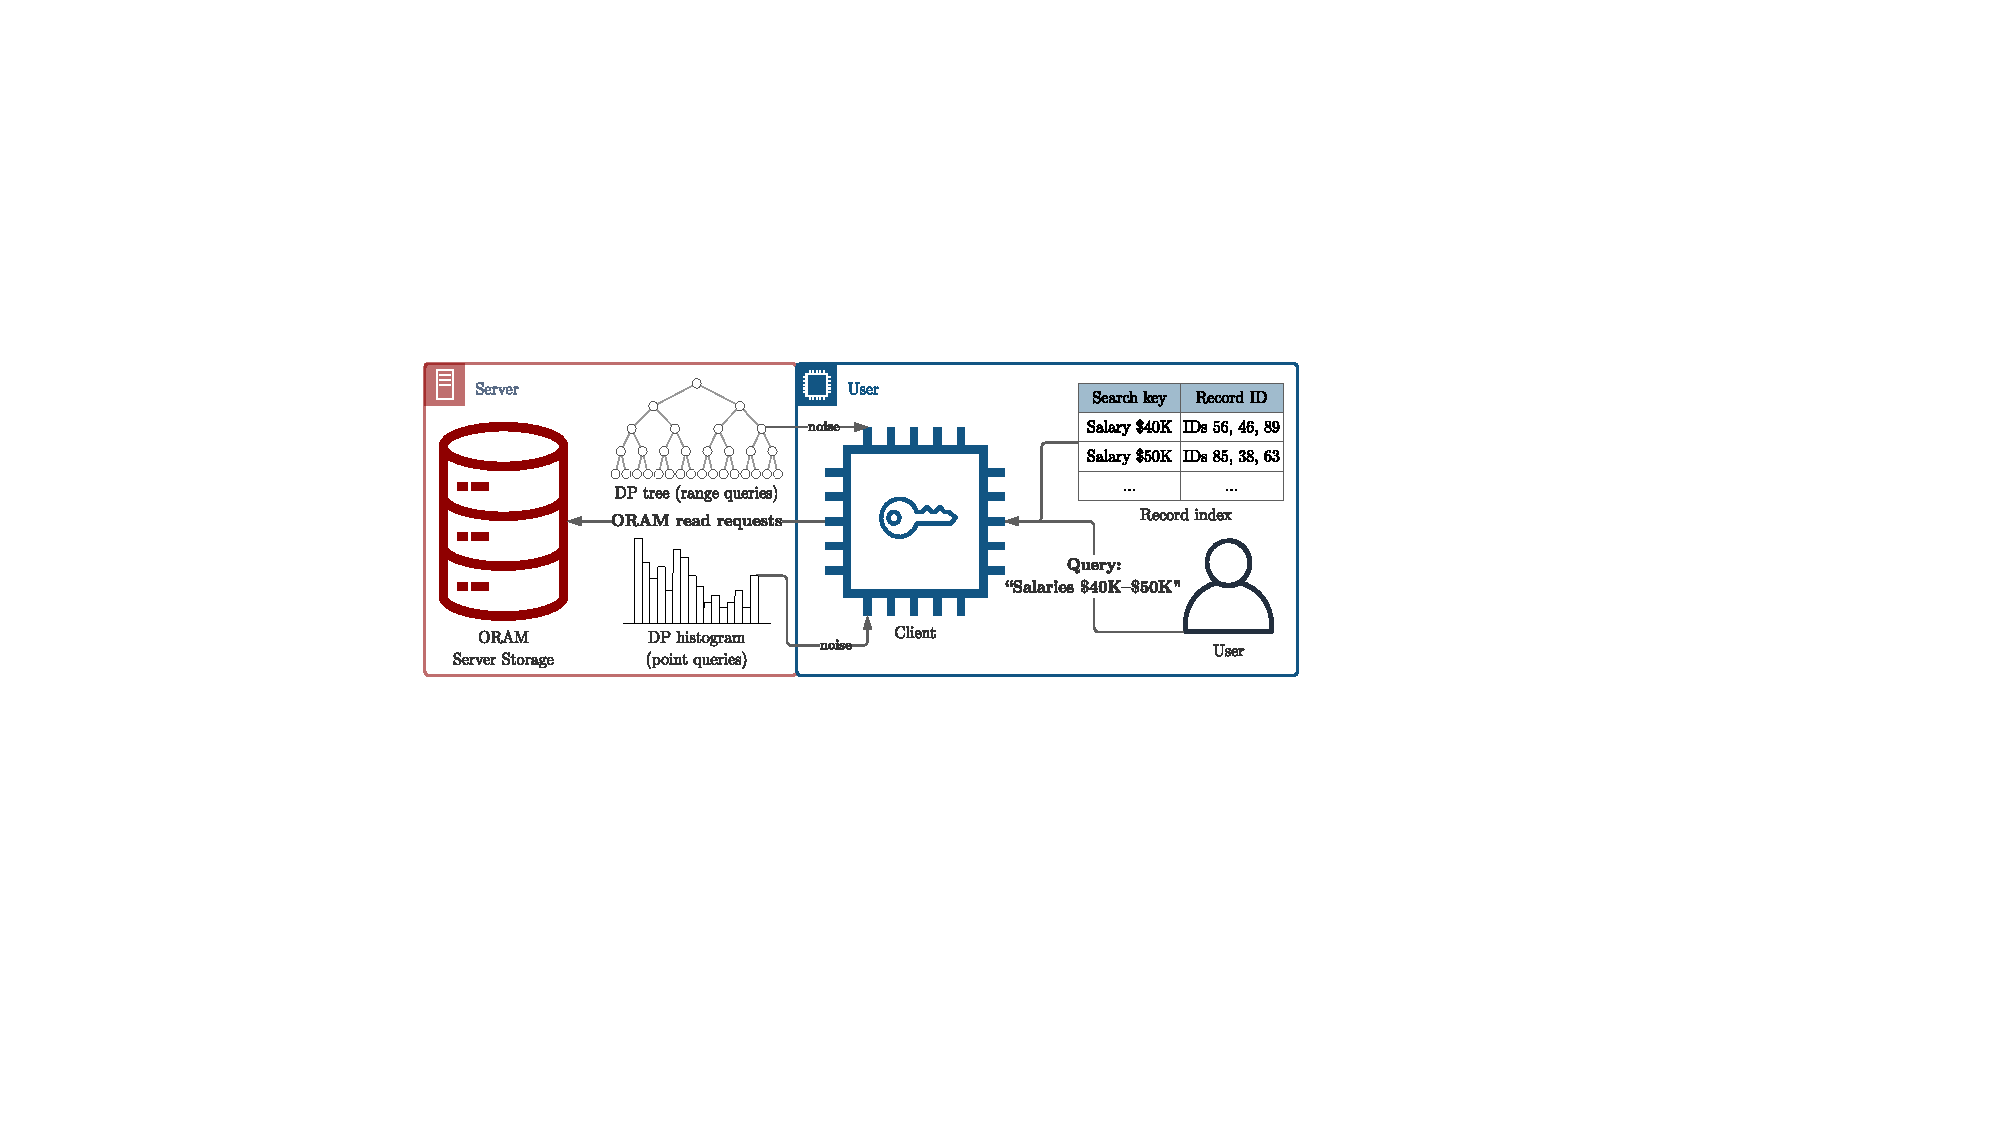
\includegraphics[width=\linewidth]{dp-oram}
	\caption{\epsolute{} construction}%
	\label{figure:dp-oram}
\end{figure}


	\subsection{Security}

		\begin{theorem}
			\epsolute{} is $(\beta \cdot m)$-wrong and $(\epsilon, \delta)$-\acrshort{cdpodb} where the negligible term is $\negl = 2 \cdot \eta_2$.
		\end{theorem}

		\begin{proof}
			We consider a sequence of views
			\[
				\view{1} \to \view{2} \to \view{3} \to \view{4} \; .
			\]
			\view{1} is \view{\protocol}{\database, \fromNtoM{\query}{1}{m}}.
			\view{2} is produced only from $\serverDS \gets \algo{A}{\fromNtoM{\searchKey}{1}{\domainSize}}$.
			Namely, compute $c_i \gets \algo{A}{\serverDS, \query_i}$ for all $i$ and run \acrshort{oram} simulator on $\sum_i c_i$.
			By \acrshort{oram} security,
			\[
				\probability{\adversary(\view{1})} - \probability{\adversary(\view{2})} \leq \eta_2 \; .
			\]
			\view{3} is produced similarly but $\serverDS \gets \algo{A}{\fromNtoM{\searchKey^\prime}{1}{\domainSize}}$ instead.
			Note that the $c_i$ are simply post-processing on \serverDS{} via \algo{B} so
			\[
				\probability{\adversary(\view{2})} = \exp(\epsilon) \cdot \probability{\adversary(\view{3})} + \delta \; .
			\]
			$\view{4} = \view{\protocol}{\database^\prime, \fromNtoM{\query}{1}{m}}$.
			It follows by \acrshort{oram} security
			\[
				\probability{\adversary(\view{3})} - \probability{\adversary(\view{4})} \leq \eta_2 \; .
			\]
			Putting this all together completes the proof.
		\end{proof}

	\subsection{Efficiency}

		For an \acrshort{oram} with communication efficiency $(a_1, a_2)$ and an $(\alpha, \beta)$-differentially private sanitizer, the \epsolute{} communication efficiency is $(a_1, a_2 \cdot \alpha)$.
		The efficiency metrics demonstrate how the total storage or communication volume (the number of stored or transferred bits) changes additively and multiplicatively as the functions of data size \dataSize{} and domain \domainSize{}.
		We therefore have the following corollaries for the efficiency of the system in the cases of approximate and pure differential privacy.
		\begin{corollary}\label{corollary:comm-efficiency-approximate-dp}
			\epsolute{} is an outsourced database system with storage efficiency \efficiency{1}{0}.
			Depending on the query type, assume it offers the following communication efficiency.
			\begin{description}
				\item[Range queries] $\efficiency{\log \dataSize}{2^{\log^* \domainSize} \log \dataSize}$
				\item[Point queries] $\efficiency{\log \dataSize}{\log \dataSize}$
			\end{description}
			Then, there is a negligible $\delta$ such that \epsolute{} satisfies $(\epsilon, \delta)$\hyp{}differential privacy for some $\epsilon$.\footnote{
				Note that the existence of $\epsilon$ in this setting implies that the probability of an adversary breaking the \acrshort{dp} guarantees is bounded by it.
			}
		\end{corollary}

		\begin{proof}
			By using \acrshort{oram}, we store only the original data once and hence, we get optimal storage efficiency.

			The communication efficiency depends on the upper bound of the error for each sanitizer when $\delta > 0$, as described in \cref{section:range-persistent:building-blocks:dp} and \cref{remark:dp-sanitizer-guarantees}.
			The most efficient \acrshort{oram} protocol to date has $\bigO{\log \dataSize}$ communication overhead (see \cref{section:range-persistent:building-blocks:oram}).
		\end{proof}

		\begin{corollary}\label{corollary:comm-efficiency-pure-dp}
			\epsolute{} is an outsourced database system with storage efficiency \efficiency{1}{0}.
			Depending on the query type, assume it offers the following communication efficiency.
			\begin{description}
				\item[Range queries] $\efficiency{\log \dataSize}{\log \domainSize \log \dataSize}$
				\item[Point queries] $\efficiency{\log \dataSize}{\log \domainSize \log \dataSize}$
			\end{description}
			Then, \epsolute{} satisfies $\epsilon$-differential privacy for some $\epsilon$.
		\end{corollary}

		\begin{proof}
			Similarly, we derive the proof by considering the use of \acrshort{oram} and the upper bound of the error for each sanitizer when $\delta = 0$ in \cref{section:range-persistent:building-blocks:dp}.
		\end{proof}

	\subsection{Extending to multiple attributes}\label{section:range-persistent:dp-oram:multiple-attributes}

		We will now describe how \epsolute{} supports multiple indexed attributes and what the privacy and performance implications are.
		The na\"{\i}ve way is to simply duplicate the entire stack of states of \user{} and \server{}, and during the query use the states whose attribute the query targets.
		However, \epsolute{} design allows to keep the most expensive part of the state --- the \acrshort{oram} state --- shared for all attributes and both types of queries.
		Specifically, the index \indexI{} and \acrshort{dp} structure \serverDS{} are generated per attribute and query type, while \user{} and \server{} \acrshort{oram} states are generated once.
		This design is practical since \serverDS{} is tiny and index \indexI{} is relatively small compared to \acrshort{oram} states, see \cref{section:range-persistent:experiments}.

		We note that in case the indices grow large in number, it is practical to outsource them to the adversarial server using \acrshort{oram} and download only the ones needed for each query.
		In terms of privacy, the solution is equivalent to operating different \epsolute{} instances because \acrshort{oram} hides the values of records and access patterns entirely.
		Due to \cref{theorem:composition} for non-disjoint datasets, the total privacy budget of the multi-attribute system will be the sum of individual budgets for each attribute / index.

		Next, we choose two \acrshort{dp} sanitizers for our system, for point and for range queries, and calculate the $\alpha$ values to make them output positive values with high probability, consistent with \cref{remark:dp-sanitizer-guarantees}.

	\subsection{\texorpdfstring{\epsolute{}}{Epsolute} for point queries}\label{section:range-persistent:dp-oram:point}

		For point queries, we use the \acrshort{lpa} method as the sanitizer to ensure pure differential privacy.
		Specifically, for every histogram bin, we draw noise from the Laplace distribution with mean $\alpha_p$ and scale $\lambda = \nicefrac{1}{\epsilon}$.
		To satisfy \cref{remark:dp-sanitizer-guarantees}, we have to set $\alpha_p$ such that if values are drawn from $\algo{Laplace}{ \alpha_p, \nicefrac{1}{\epsilon} }$ at least as many times as the number of bins \domainSize{}, they are all positive with high probability $1 - \beta$, for negligible $\beta$.

		We can compute the exact minimum required value of $\alpha_p$ in order to ensure drawing positive values with high probability by using the \acrshort{cdf} of the Laplace distribution.
		Specifically, $\alpha_p$ should be equal to the minimum value that satisfies the following inequality.

		\[
			\left( 1 - \frac{1}{2} e^{- \alpha_p \cdot \epsilon} \right)^\domainSize \leq 1 - \beta
		\]
		which is equivalent to
		\[
			\alpha_p = \ceil{ -\frac{ \ln \left( 2 - 2 \sqrt[\domainSize]{1 - \beta} \right) }{ \epsilon } }
		\]

	% chktex-file 1
% chktex-file 8
% chktex-file 21
% chktex-file 24
% chktex-file 26
% chktex-file 36
% chktex-file 37

\setlength{\setupLength}{16em}
\setlength{\queryLength}{15em}

\newcommand{\SetupGamma}{
	\procedure[linenumbering]{\protocolSetup{} of \protocolGamma{}}{
																\textbf{User \user}																							\>																\> \textbf{Server \server}	\\
		%
		\label{algorithm:dp-oram-parallel:gamma:setup:line-2}	\pcinput{\database{}}																						\>																\> \pcinput{\emptyset}		\\
		%
		\label{algorithm:dp-oram-parallel:gamma:setup:line-3}	\indexI \gets \algo{CreateIndex}{\database, \oramsNumber}													\>																\>							\pclb
		%
		\pcintertext[dotted]{$\pcfor j \in \set{1, \ldots, \oramsNumber} \pcdo$ \; \text{(in parallel)}}
		%
		\label{algorithm:dp-oram-parallel:gamma:setup:line-4}	\left\langle \overline{\record}, \overline{\recordID} \right\rangle\ \text{s.t.}\ \algo{H}{\recordID} = j	\>																\>							\\
		%
		\label{algorithm:dp-oram-parallel:gamma:setup:line-5}	\oramProgram = \left\langle (\oramWrite, \overline{\recordID}, \overline{\record}) \right\rangle			\> \sendmessageboth*[\setupLength]{\algo{ORAM}_j(\oramProgram)}	\>							\pclb
		%
		\pcintertext[dotted]{$\pcendfor$}
		%
		\label{algorithm:dp-oram-parallel:gamma:setup:line-6}	\serverDS \gets \algo{A}{\fromNtoM{\searchKey}{1}{\domainSize}}												\> \sendmessageright*[\setupLength]{\serverDS}					\>							\\
		%
		\label{algorithm:dp-oram-parallel:gamma:setup:line-7}	\pcouput{\indexI}																							\>																\> \pcouput{ \serverDS }
	}
}

\newcommand{\QueryGamma}{
	\procedure[linenumbering]{\protocolQuery{} of \protocolGamma{}}{
																\textbf{User \user}																					\>																												\> \textbf{Server \server}									\\
		%
		\label{algorithm:dp-oram-parallel:gamma:query:line-2}	\pcinput{\query, \indexI}																			\>																												\> \pcinput{ \serverDS }									\\
		%
		\label{algorithm:dp-oram-parallel:gamma:query:line-3}	\fromNtoM{T}{1}{\oramsNumber} \gets \algo{Lookup}{I, \query}										\> \sendmessageright*[\queryLength]{\query}																		\> k \gets \algo{B}{\serverDS, \query}						\\
		%
		\label{algorithm:dp-oram-parallel:gamma:query:line-4}																										\> \sendmessageleft*[\queryLength]{c}																			\> c \gets (1 + \gamma) \frac{\tilde{k}_0}{\oramsNumber}	\pclb
		%
		\pcintertext[dotted]{$\pcfor j \in \set{1, \ldots, \oramsNumber} \pcdo$ \; \text{(in parallel)}}
		%
		\label{algorithm:dp-oram-parallel:gamma:query:line-5}	\oramProgram_\mathsf{true} = \left. (\oramRead, \recordID_i, \bot) \right|_{i \in T_j}				\>																												\>															\\
		%
		\label{algorithm:dp-oram-parallel:gamma:query:line-6}	\oramProgram_\mathsf{noise} = \left. (\oramRead, S \setminus T_j, \bot) \right|_{1}^{c - \abs{T_j}}	\> \sendmessageboth*[\queryLength]{\algo{ORAM}_j(\oramProgram_\mathsf{true} \| \oramProgram_\mathsf{noise})}	\> R_j														\pclb
		%
		\pcintertext[dotted]{$\pcendfor$}
		%
		\label{algorithm:dp-oram-parallel:gamma:query:line-7}	\pcouput{ \left. R_j \right|_{j = 1}^\oramsNumber }													\>																												\>	\pcouput{\emptyset}
	}
}

\begin{algorithm*}[ht!]

	\begin{pcvstack}

		\begin{pcvstack}

			\SetupGamma{}

			\vspace{0.5em}

			\QueryGamma{}

		\end{pcvstack}

	\end{pcvstack}

	\caption[Parallel \epsolute{} for \protocolGamma{}]{
		Parallel \epsolute{} for \protocolGamma{}, extends \cref{algorithm:dp-oram}.
		\algo{H} is a random hash function $\algo{H} : \bin^* \to \set{1, \ldots, \oramsNumber}$.
		$\gamma$ and $\tilde{k}_0$ are computed as in \cref{section:range-persistent:prallel-dp-oram:gamma}.
	}%
	\label{algorithm:dp-oram-parallel}
\end{algorithm*}


	\subsection{\texorpdfstring{\epsolute{}}{Epsolute} for range queries}\label{section:range-persistent:dp-oram:range}

		For range queries, we implement the aggregate tree method as the sanitizer.
		Specifically, we build a complete \fanout{}-ary tree on the domain, for a given \fanout{}.
		A leaf node holds the number of records falling into each bin plus some noise.
		A parent node holds sum of the leaf values in the range covered by this node, plus noise.
		Every time a query is issued, we find the minimum number of nodes that cover the range, and determine the required number of returned records by summing these node values.
		Then, we ask the server to retrieve the records in the range, plus to retrieve multiple random records so that the total number of retrieved records matches the required number of returned records.

		The noise per node is drawn from the Laplace distribution with mean $\alpha_h$ and scale $\lambda = \frac{\log_{\fanout} \domainSize}{\epsilon}$.
		Consistent with \cref{remark:dp-sanitizer-guarantees}, we determine the mean value $\alpha_h$ in order to avoid drawing negative values with high probability.
		We have to set $\alpha_h$ such that if values are drawn from $\algo{Laplace}{ \alpha_h, \frac{\log_{\fanout} \domainSize}{\epsilon} }$ at least as many times as the number of nodes in the tree, they are all positive with high probability $1 - \beta$, for negligible $\beta$.

		Again, we can compute the exact minimum required value of $\alpha_h$ in order to ensure drawing positive values with high probability by using the \acrshort{cdf} of the Laplace distribution.
		Specifically, $\alpha_h$ should be equal to the minimum value that satisfies the following inequality.
		\[
			\left( 1 - \frac{1}{2} e^{- \frac{\alpha_h \cdot \epsilon}{\log_{\fanout} \domainSize}} \right)^\mathsf{nodes} \leq 1 - \beta
		\]
		which is equivalent to
		\begin{equation}\label{equation:min-mu-for-range}
			\alpha_h = \ceil{ -\frac{ \ln{ (2 - 2 \sqrt[\mathsf{nodes}]{ 1 - \beta } ) } \cdot \log_{\fanout} \domainSize }{\epsilon} }
		\end{equation}
		where $\mathsf{nodes} = \frac{ \fanout^{ \ceil{ \log_{\fanout} (\fanout - 1) + \log_{\fanout} \domainSize - 1 }} - 1}{ \fanout - 1 } + \domainSize$ is the total number of tree nodes.
